%%%%%%%%%%%%%%%%%%%%%%%%%%%%%%%%%%%%%%%%%%%%%%%%%%%%%%%%%%
%% Dynawo validation project: Final Report
%%
%% (c) 2020 Grupo AIA for RTE
%%
%% Contact author: marinjl@aia.es
%%
%%
%%
\documentclass[11pt, a4paper, twoside, titlepage]{article}
\usepackage[utf8]{inputenc}
\usepackage{amsmath}
\usepackage{amssymb}
\usepackage{graphicx}
\usepackage[export]{adjustbox} % for valign=c in includegraphics
\usepackage{booktabs}
\usepackage{listings}
\usepackage{xcolor}
\usepackage{fancyvrb}
\usepackage[hidelinks]{hyperref} 

%%%%%%%%%%%%%%%%%%%%%%%%%%%%%%%%%%%%%%%%%%%%%%%%%%%%%%%%%%%
%%% Fancy headings
%%%%%%%%%%%%%%%%%%%%%%%%%%%%%%%%%%%%%%%%%%%%%%%%%%%%%%%%%%%
\usepackage{fancyhdr}
\setlength{\headheight}{15pt}  % needs to be 13.6pt or more
\pagestyle{fancy}
%\renewcommand{\chaptermark}[1]{ \markboth{#1}{} }
\renewcommand{\sectionmark}[1]{\markboth{#1}{}}
\fancyhf{}
\fancyhead[LE]{\textit{\nouppercase{\leftmark}}}
\fancyhead[RO]{\textit{\nouppercase{\rightmark}}}
\fancyfoot[LE,RO]{\bfseries\thepage}
\fancyfoot[RE]{\textsc{\small Dynawo validation report}%
  \phantom{I}
\includegraphics[width=0.6cm,valign=c]{logos/Logo-pequeno.png}}
\fancyfoot[LO]{
\includegraphics[width=0.6cm,valign=c]{logos/Logo-pequeno.png}%
  \phantom{I}\textsc{\small Dynawo validation report}}
\renewcommand{\headrulewidth}{0.4pt}
\renewcommand{\footrulewidth}{0.4pt}
\addtolength{\footskip}{\baselineskip}
%% \fancypagestyle{plain}{ %
%%   \fancyhf{} % remove everything
%%   \renewcommand{\headrulewidth}{0pt} % remove lines as well
%%   \renewcommand{\footrulewidth}{0pt}
%% }


% Our colors for backgrounds and code listings
\definecolor{light-gray}{gray}{0.9}
\definecolor{dark-gray}{gray}{0.4}
\definecolor{light-blue}{RGB}{64,64,255}
\definecolor{dark-blue}{RGB}{16,16,64}

\lstset{% config parameters for code listings
  language=Python,
  backgroundcolor=\color{light-gray},
  basicstyle=\scriptsize\ttfamily,
  keywordstyle=\bfseries,
  identifierstyle=,
  stringstyle=\itshape,
  showstringspaces=false,
  commentstyle=\color{dark-gray}
}


%%% Various other settings and short-hand macros
\lstnewenvironment{console}{\lstset{language=bash}}{}
\newcommand{\code}[1]{\texttt{#1}}

\hypersetup{
  colorlinks = true, % color links instead of ugly boxes
  urlcolor   = blue, % color of external hyperlinks
  linkcolor  = dark-blue, % color of internal links
  citecolor  = red   % color of citations
}





%%%%%%%%%%%%%%%%%%%%%%%%%%%%%%%%%%%%%%%%%%%%%%%%%%%%%%%%%%
%%% Document starts here
%%%%%%%%%%%%%%%%%%%%%%%%%%%%%%%%%%%%%%%%%%%%%%%%%%%%%%%%%%

\title{Dynawo validation: Final Report}
\author{José Luis Marín, Vicenç Gaitán \\
	Grupo AIA for RTE}

\date{
  \vspace{2cm}
  
\includegraphics[width=2cm]{logos/Logo_RTE.pdf}
  
\includegraphics[width=2cm]{logos/Logo-pequeno.png}\\
  \vspace{1cm}
  30 December 2020
} 


\begin{document}

\hypersetup{pageanchor=false}
\begin{titlepage}
  \maketitle
\end{titlepage}
\hypersetup{pageanchor=true}

\begin{abstract}
  This report documents the work carried out by Grupo AIA in the
  Project \emph{``Validation de Dynawo estabilité en tension''} for
  RTE. The goal of this project is to quantitatively assess Dynawo for
  long-term stability simulations (\emph{``DynaWaltz''}), using RTE's
  models and cases. The overall approach to this project, as suggested
  by RTE, has been the use of another well-established simulator,
  \emph{Astre}, as the reference for comparison and assessment.  This
  is a practical starting point for validation that can later be
  incrementally augmented with comparisons to real field data (which
  are typically harder to get). More specifically, the validation
  efforts have been focused on the results obtained for the behavior of
  the coordinated Secondary Voltage Control systems.

  The work obviously has \emph{not} been a one-off, pass/not-pass
  validation study; instead, we developed a software tool for the
  rapid preparation, simulation, and analysis of multiple
  (contingency) test cases, usable for any forthcoming versions of
  DynaWaltz and for any changes in the grid cases. As it is, the tool
  has been built to compare Dynawo vs.\ Astre, but with suitable
  modifications it could be used to compare Dynawo version A
  vs.\ Dynawo version B, which will certainly be useful for the
  ongoing development of Dynawo and RTE models.

  After presenting a description of the general approach, the bulk of
  this report is dedicated to: (a) specifying the validation criteria,
  i.e. the definition of \emph{characterizing measures} and the
  associated \emph{metrics} with which the results are compared, which
  is at the heart of the methodology; (b) providing a detailed manual
  with technical requirements, installation, and operating instructions
  for using the software tools.
  
  The report also contains some notes for developers, with pointers to
  the specific parts of the code on the GitHub repository, where all
  the code and documentation is kept.
\end{abstract}



\tableofcontents

\section{Introduction}

\subsection{The project}
This report documents the work carried out by Grupo AIA in the Project
\emph{``Validation de Dynawo estabilité en tension''} (RTE
ref.\ no.\ 4500717774). The project was carried out in July--December
of 2020.

The stated goal of the project is to provide support to RTE in the
validation of dynamic simulations made using the open source tool
Dynawo (in the context of long-term stability simulations), verifying
that results obtained for the provided test cases are realistic and
that the modeled power system behaves in the expected way from a
physical point of view.

Dynawo is a hybrid C++/Modelica open-source time-domain simulation
tool for power systems, in which RTE has played a major role in
development. It is an ongoing project based on previous work conducted
particularly in two R\&D European projects: Pegase and iTesla.  These
projects contributed to the foundational designs of Dynawo, since they
demonstrated the usability of the Modelica language for power system
simulations and contributed to the development of numerical resolution
strategies that are now integrated into Dynawo.

As a time-domain simulator, Dynawo is quite versatile and contains
several solvers, thanks to which it can cover many different time
scales, from long-term stability to quasi-EMT. Additionally, this
Modelica-based approach is being extended to other
functionalities. Starting in July 2020, Dynawo is evolving towards a
complete and coherent suite of simulation tools, all sharing the same
philosophy:
\begin{description}
\item[DynaFlow] for steady-state calculations
\item[DySym] for short-circuit calculations
\item[DynaWaltz] for long-term stability simulations
\item[DynaSwing] for short-term stability studies
\item[DynaWave] for stability studies and system design with a
  high-penetration of power-electronics based components (quasi-EMT)
\end{description}
In this light, this project is focused on \emph{DynaWaltz}, and more
specifically, on the validation of RTE's private version of the
DynaWaltz software, applied to RTE's grid models. Particular emphasis
is to be placed in the simulation fidelity of the coordinated
Secondary Voltage Control systems, SVC (RST in French), which is key
for long-term stability at the network-wide scale.


\subsection{Structure of this report}
This report is structured as follows. In Section~\ref{sec:approach} we
describe the general approach taken to tackle this project, which was
\emph{not} simply a one-off, pass/not-pass validation study; instead,
we developed a software tool for the rapid preparation, simulation,
and analysis of multiple tests, usable for any forthcoming versions of
DynaWaltz and for any changes in the grid test cases.
Section~\ref{sec:metrics} then describes the key point of the
methodology upon which we base our validation criteria, i.e. the
definition of \emph{characterizing measures} and the associated
\emph{metrics} to compare different results. These contemplate both
continuous magnitudes (``curves'') and discrete events (automata
actions).  Sections~\ref{sec:usermanual} and \ref{sec:devnotes}
contain the ``User Manual'' and ``Developer Manual'',
respectively. For the user, we try to provide a complete picture of
how to use the tool end-to-end. For developers, we describe the
overall design of the tools and then provide pointers to the specific
parts of the code on the GitHub repo. Finally,
Appendix~\ref{app:github} describes the structure of the GitHub repo
in more detail.




\section{Approach: Dynawo vs.\ Astre}
\label{sec:approach}

As suggested by RTE, the overall approach to this project is based on
the use of another well-established simulator, \emph{Astre}, as the
reference for comparison and assessment. Although, ideally, one would
like to compare simulation results against real field data, these are
typically harder to get. Therefore, comparing against Astre is a
pragmatic and effective starting point for validation. Additionally,
using a second simulator allows testing extensively many cases, far
more than those available in the experimental data---for instance,
running an exhaustive list of contingencies.

This validation against Astre has not been performed as a one-off
study with a given list of test cases. Instead, we developed a
complete system that automates almost all of the steps involved in
performing a comparison of results: the preparation of cases, running
the simulations, extracting the relevant data from the output, and
analyzing the results.  The software is usable for any forthcoming
versions of DynaWaltz and for any changes in the grid test cases.
Another way in which the software may be used is by analyzing how two
different versions of Dynawo compare against Astre (which is no longer
being developed and therefore static).  Future developments of this
software may be aimed in the direction of directly comparing Dynawo
version A vs.\ Dynawo version B, which could be useful for the ongoing
development of Dynawo and RTE models.

The test cases are constructed as all possible single-element
\emph{contingency} cases, which is actually one of the main use cases
that RTE has in mind for deploying DynaWaltz in production. The
software provides a mechanism to limit the amount of contingency cases
via random sampling, if CPU/storage resources were limited (or if
someone simply wants to run a non-exhaustive check).

The validation criteria have been focused on the results obtained for
the behavior of the coordinated Secondary Voltage Control
systems. This means that, among the huge number of all possible
signals (network variables) available from the simulation, the
comparison looks only at these:
\begin{itemize}
\item the pilot voltages, K-levels, and (P,Q) of generators
  participating in SVC controls
\item the bus voltage(s) of bus(es) involved in the particular
  contingency
\end{itemize}
However, the criteria also contemplate certain automata events
(transformer tap changers, shunts connections/disconnections), with no
restriction on which part of the network they come from.  The base
test cases correspond to the seven SVC zones in RTE's network (Lille,
Lyon, Marseille, Paris, Nancy, Nantes, and Toulouse), plus an
additional case for the whole of France.

The data from all of these signals, both continuous and discrete, are
then ``distilled'' into a handful of reduced magnitudes (such as
peak-to-peak, period, etc.). This way the full time-dependent curve
(or the sequence of events, in the case of automata) gets reduced into
a few values that characterize the signal. It is then on these
magnitudes that we define certain metrics, in order to quantify the
comparison between Astre and Dynawo results. These multiple metrics
are in turn combined into one or more compound scores, which can be
used to rank the contingency cases.  For the full details about the
definition of these metrics and compound scores, see
Section~\ref{sec:metrics} below.

To recapitulate, the approach can be briefly summarized as:
\begin{itemize}
\item validating DynaWaltz by comparison against Astre
\item by running over all single-element contingency cases
\item focusing on SVC, by selecting all SVC-related variables (pilot
  V, K-levels, P\&G of participating gens)
\item and also considering the bus V at contingency points
\item extracting relevant magnitudes from these particular curve
  signals (steady-state net change, peak-to-peak amplitude, etc.)
\item and extracting relevant events from \emph{all} automata actions
  (transformer taps, shunts)
\item defining \emph{metrics} on all those extracted data (curves and
  automata events) and \emph{compound scores} for ranking cases
\item and finally, materializing all this in the construction of an
  automated tool (processing pipeline) and a quick analysis \&
  assessment tool (notebook).
\end{itemize}




\section{The design of metrics and thresholds for validation}
\label{sec:metrics}

Since the approach of this project is based on extensive
\emph{quantitative} comparison between Astre and Dynawo in medium to
long-term stability simulations of contingency cases, we need to lay
down the comparison criteria with precision. To break down the
complexity of the whole process, it is useful to adopt the following
conceptual itinerary:
\begin{enumerate}
  \item One should begin by selecting the \emph{``signals''} to be
    used for the comparison. Which output variables and events should
    be considered and which should be discarded? --- Because it's simply
    not manageable nor practical to compare all of them.
  \item Then generate a suitable \emph{reduced set of parameters} that
    characterize each type of signal.  Because one is not interested
    in perfect waveform accuracy (in the case of curves), or in
    perfect event timings (in the case of automata events).
  \item Then design the \emph{metrics} for measuring the distance
    between Astre and Dynawo results in the space of those reduced
    parameters.
  \item And finally, define validation \emph{thresholds} for each
    class of such metrics, and possibly one or more \emph{compound
      scoring} schemes for ranking cases. The thresholds are useful in
    order to estabish hard pass / not-pass criteria for validating
    DynaWaltz. And compound scores are needed because the reduced
    parameters are of very disparate classes (say, for instance,
    change in bus voltage steady state versus Mvar peak-to-peak
    amplitude, versus number of tap changer events); therefore we need
    to decide how to combine these into a single figure of merit, for
    the purposes of ranking and sifting the worst cases that need our
    attention.
\end{enumerate}

We now go over each one of these in more detail.

\subsection{Selection of signals}

Here we use the word \emph{signals} to refer to both time-dependent continuous
variables such as voltages and (P,Q) values, as well as discrete events such as
actions fired by control automata.  Many times we will refer to signals of the
first kind as \emph{``curves''}, since this is the terminology used for the
output in both Astre and Dynawo. For signals of the second kind, we will simply
call them \emph{``automata events''} or simply automata.

By common agreement with RTE, and because the validation needs to
focus especially on the coordinated Secondary Voltage Control systems
(RST, in French), we have selected the following signals:
\begin{itemize}
\item Curve magnitudes:
  \begin{itemize}
  \item Voltages of the SVC pilot buses
  \item K-levels of the SVC
  \item P, Q of generators participating in the SVC (but only for SVCs belonging
    to the relevant Area)
  \item Voltage(s) of the bus(es) affected by the contingency 
  \end{itemize}
\item Automata events:
  \begin{itemize}
  \item Shunt connections / disconnections --- anywhere
  \item Transformer taps (up / down) --- anywhere
  \item Load-transformer taps (up / down) --- anywhere
  \end{itemize}  
\end{itemize}

Note that K-levels are discrete in nature and each change of their value also
appears in the output as events, but it is much easier to deal with them as
curve data.


\subsection{Reduced set of parameters}

Here the aim is to distill a reduced set of parameters that characterize the
whole signal sufficiently well for our purposes. Since these are transient
signals and we are not really interested in matching the detailed waveforms with
high fidelity, we came up with the following parameters.

Reduced parameters for curves:

\begin{description}
\item[dSS:] \hfill \\ ``delta-SS'', i.e. the difference in signal value between
  the initial steady state and the final steady state.
\item[dPP:] \hfill \\ ``delta-PP'', i.e. the peak-to-peak amplitude of the
  signal during the transient.
\item[TT:] \hfill \\ transient time, i.e. the duration of the transient.
\item[period:] \hfill \\ period of the main component of the transient, as
  obtained by Prony analysis.
\item[damping:] \hfill \\ damping of the main component of the transient, as
  obtained by Prony analysis.
\end{description}

For automata events, and more precisely for tap and shunt events, we have
devised a reduced set of 3 parameters that mimic dSS, dPP, and TT, respectively:

\begin{description}
\item[netchange:] \hfill \\ net change in tap value (or in connection status,
  for shunts) between the initial steady state and the final steady state.
\item[p2pchange:] \hfill \\ peak-to-peak change in tap value during the
  transient.
\item[numchange:] \hfill \\ total number of tap changes (or connection /
  disconnections, for shunts) in the transient.
\end{description}

Figures~\ref{fig:tcharacteristics1} and ~\ref{fig:tcharacteristics2} below show
all these parameters graphically.

\begin{figure}
  \centering
  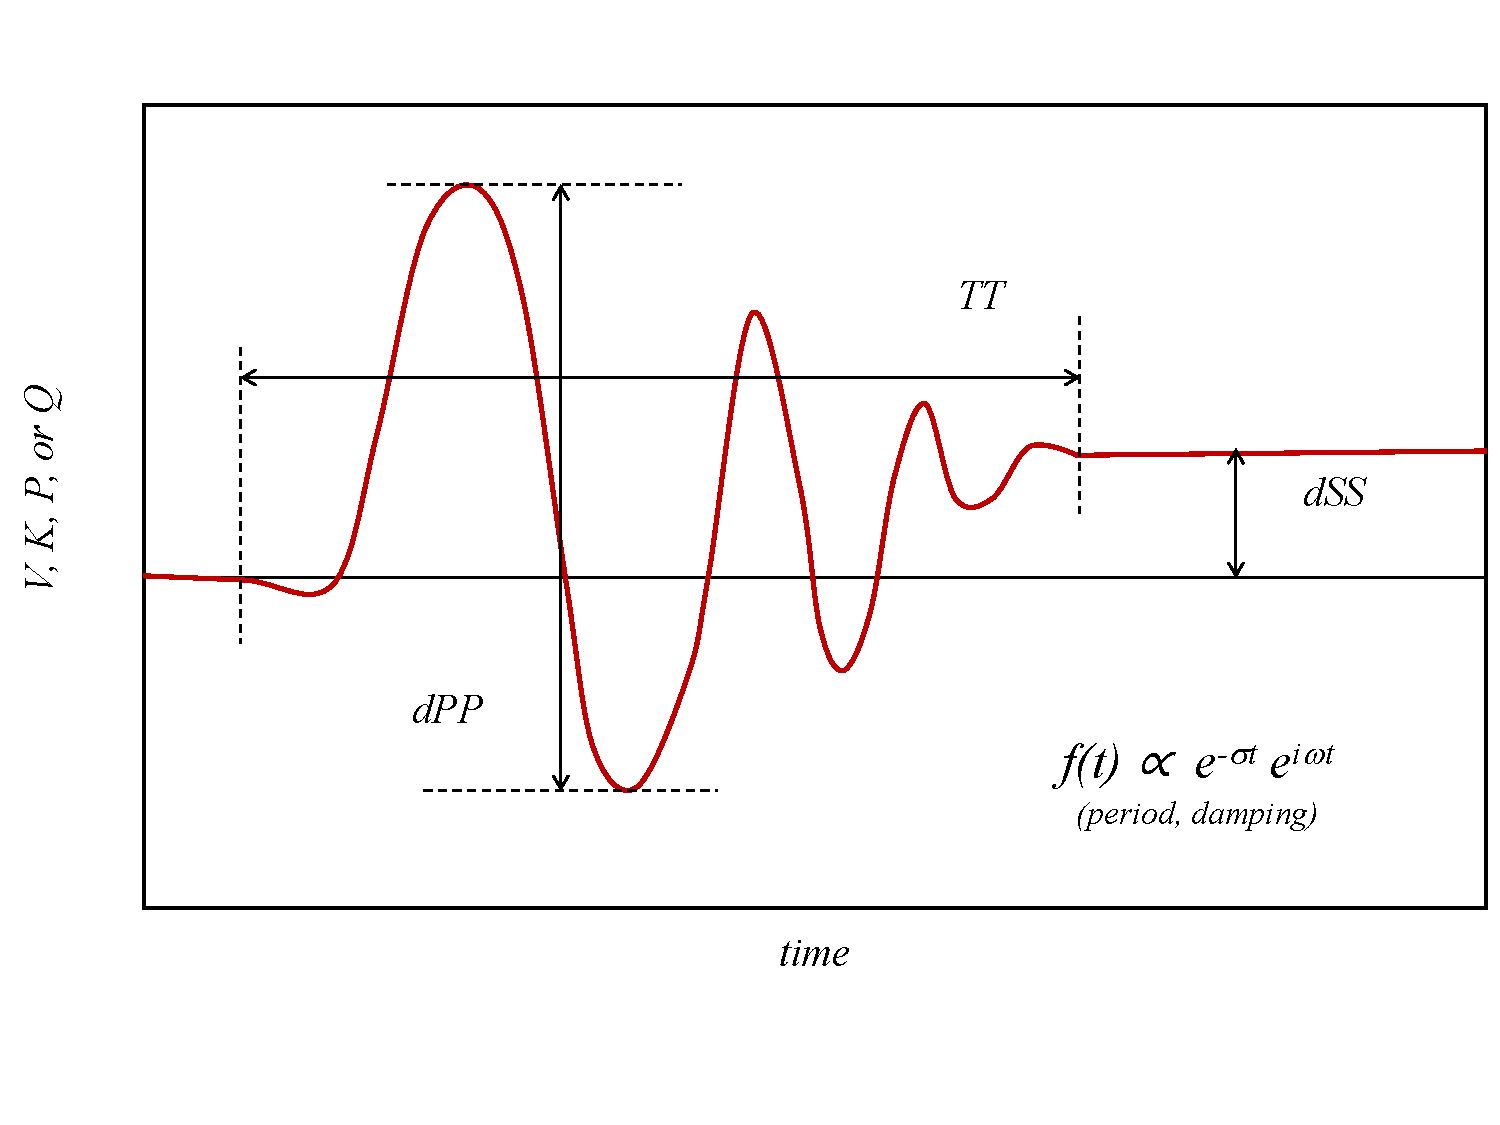
\includegraphics[width=\columnwidth]{figs/transient_characteristics_1}
  \caption{A reduced set of five parameters characterizing a continuous
    time-dependent transient signal.}
  \label{fig:tcharacteristics1}
\end{figure}

\begin{figure}
  \centering
  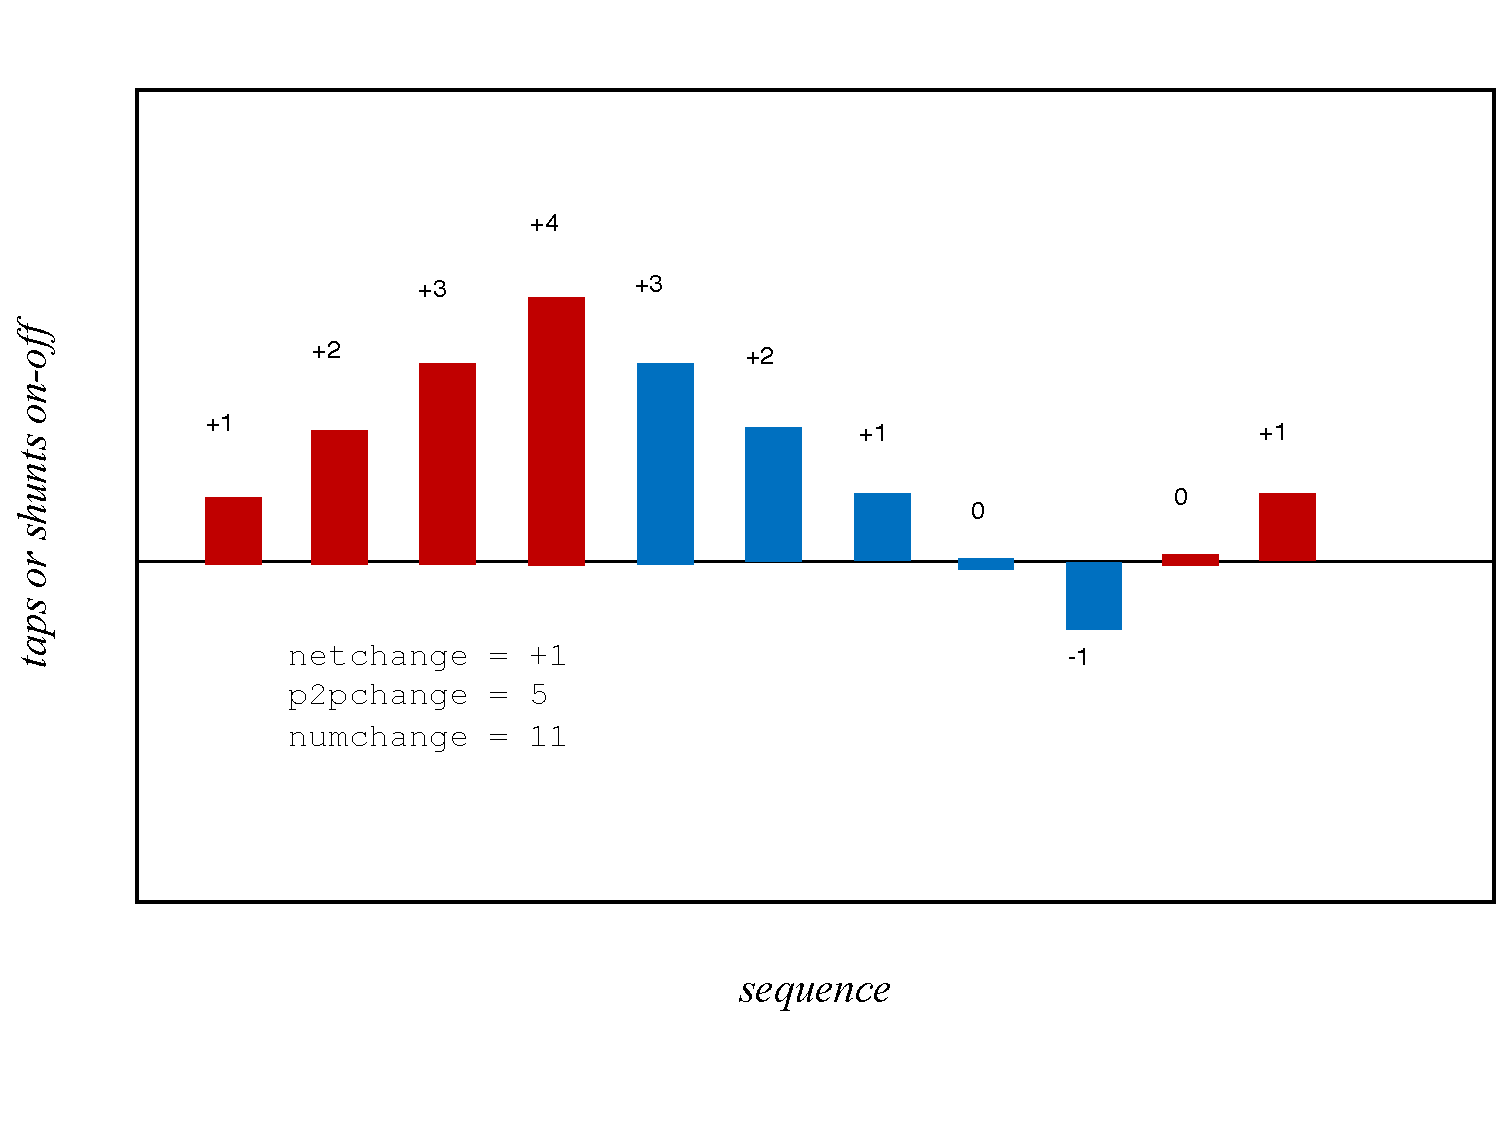
\includegraphics[width=\columnwidth]{figs/transient_characteristics_2}
  \caption{A reduced set of three parameters characterizing a sequence of binary
    (up/down, on/off) events.}
  \label{fig:tcharacteristics2}
\end{figure}



\subsection{Metrics}

%% [Here a description of how a metric is defined for each combination category of
%%   ``magnitude + reduced-parameter''. Essentially: do we use mean(abs(diffs)), or
%%   max(abs(diffs))?]

For curves, there's 25 categories (5 magnitudes x 5 parameters). In
each category, there's usually more than one data point. For instance,
if there are 4 SVC controls in the case file, there will be 4 pilot
voltages. We have to choose a metric in order to reduce the distances
to a single number. One possible choice is using max(abs(diffs)),
which is the max-norm (also called the l-infinity norm).  A different
choice could be using mean(abs(diffs)), which is like the l-1 norm
divided by the number of variables.

For automata events, there is 8 categories:
\begin{itemize}
\item shunt\_netchanges: L1-norm of netchange diffs, normalized by the number of shunts
\item shunt\_numchanges: L1-norm of numchange diffs, normalized by the number of shunts
\item tap\_netchanges: L1-norm of netchange diffs, normalized by the number of transformers
\item tap\_p2pchanges: L1-norm of p2pchange diffs, normalized by the number of transformers
\item tap\_numchanges:  L1-norm of numchange diffs, normalized by the number of transformers
\item ldtap\_netchanges:  L1-norm of netchange diffs, normalized by the number of load-transformers
\item ldtap\_p2pchanges: L1-norm of p2pchange diffs, normalized by the number of load-transformers
\item ldtap\_numchanges: L1-norm of numchange diffs, normalized by the number of load-transformers
\end{itemize}  

We can think of this ``normalized l-1 norm'' as being the same as using
mean(abs(diffs)), only that the number of variables we are using is \emph{all}
devices that could potentially produce events, not just the ones that have
actually produced events.


\subsection{Compound scoring and validation thresholds}

% TODO: expand a bit more the discussion about: (a) compound scores
% built from ``relative error'' metrics; (b) threshold metrics for
% validation, built from ``absolute error'' metrics.]}

Compounding the 25 + 8 different categories into an aggregate metric
needs to be done carefully, in order to deal with the ``apples vs. oranges''
problem. Using relative error for each category sidesteps this problem (but
brings others).  On the other hand, from the point of view of validation, it is
more natural to define a set of thresholds, one in each of those 25+8
categories, using absolute error (one may later decide whether to assign a
global pass/not-pass based on some supra-metric on each individual pass/not-pass
value).

\noindent \textbf{Thresholds for absolute errors}: Tentatively, we
have found the following thresholds to be reasonable.r
\begin{itemize}
\item V: 0.01 in pu
\item K: 0.1 (dimensionless)
\item P: 5 MW
\item Q: 5 MW
\end{itemize}

These thresholds are considered for characteristics dSS and dPP (see
columns \code{dSS\_pass} and \code{dPP\_pass} in the notebook and
reports).

However, keep in mind that if they are used for establishing a strict
a pass/not-pass criteria, then it is found that approximately up to
20\% of contingency cases fail the test. One may want to play around
with the thresholds in order to see how this percentage varies.





\section{Dynawo validation pipeline: User Manual}
\label{sec:usermanual}

\subsection{High-level description}
\label{subsec:hl_intro}
As described in Section~\ref{sec:approach}, this validation system is
based on comparing results against a well-known reference system, the
Astre simulator. The cases used for comparison are essentially all
possible single-element disconnections (shunts, lines, etc.), since
one of DynaWaltz's major use cases will be contingency studies.

The basic workflow of this system, from a functional point of view, is
as follows:
\begin{enumerate}
  \item Obtain a study case containing matching Dynawo and Astre files
    (in a standard file structure, see below)
  \item Prepare the base case: standardize the XML format and
    standardize the curves to be extracted
  \item Create the contingency cases derived from the base case
  \item Run Astre and Dynawo on the contingency cases, collecting logs
    and results into organized (and compressed) storage 
  \item Extract result data in a format common to Astre and Dynawo
    (this is for automata events, as curves have already been
    standardized in step 2)
  \item Compute metrics on the results obtained (both for curves and
    selected automata events)
  \item Use the Jupyter notebook to browse and analyze the results,
    and obtain lists of contingency cases that can be ranked according
    to various compound scores built on those metrics.
  \item Further analysis is possible using the ranked tables that the
    notebook exports to CSV files (e.g. using Excel)    
\end{enumerate}

The study case (Step 1) is the main input to this whole process, and
it is required to satisfy a minimum set of requirements (these are
detailed below in Subsection~\ref{subsec:reqmts}, along with other
technical requirements).

Beginning with Step 2, this whole workflow has been automated with a
series of Python programs and Bash shell scripts. Tied together, we
will refer to this system as the \emph{process pipeline} for
validation. This is depicted schematically in
Figure~\ref{fig:pipeline1} below.  In the following we describe this
pipeline in detail and explain how to run it either automatically or
manually step by step.

\begin{figure}
  \centering
  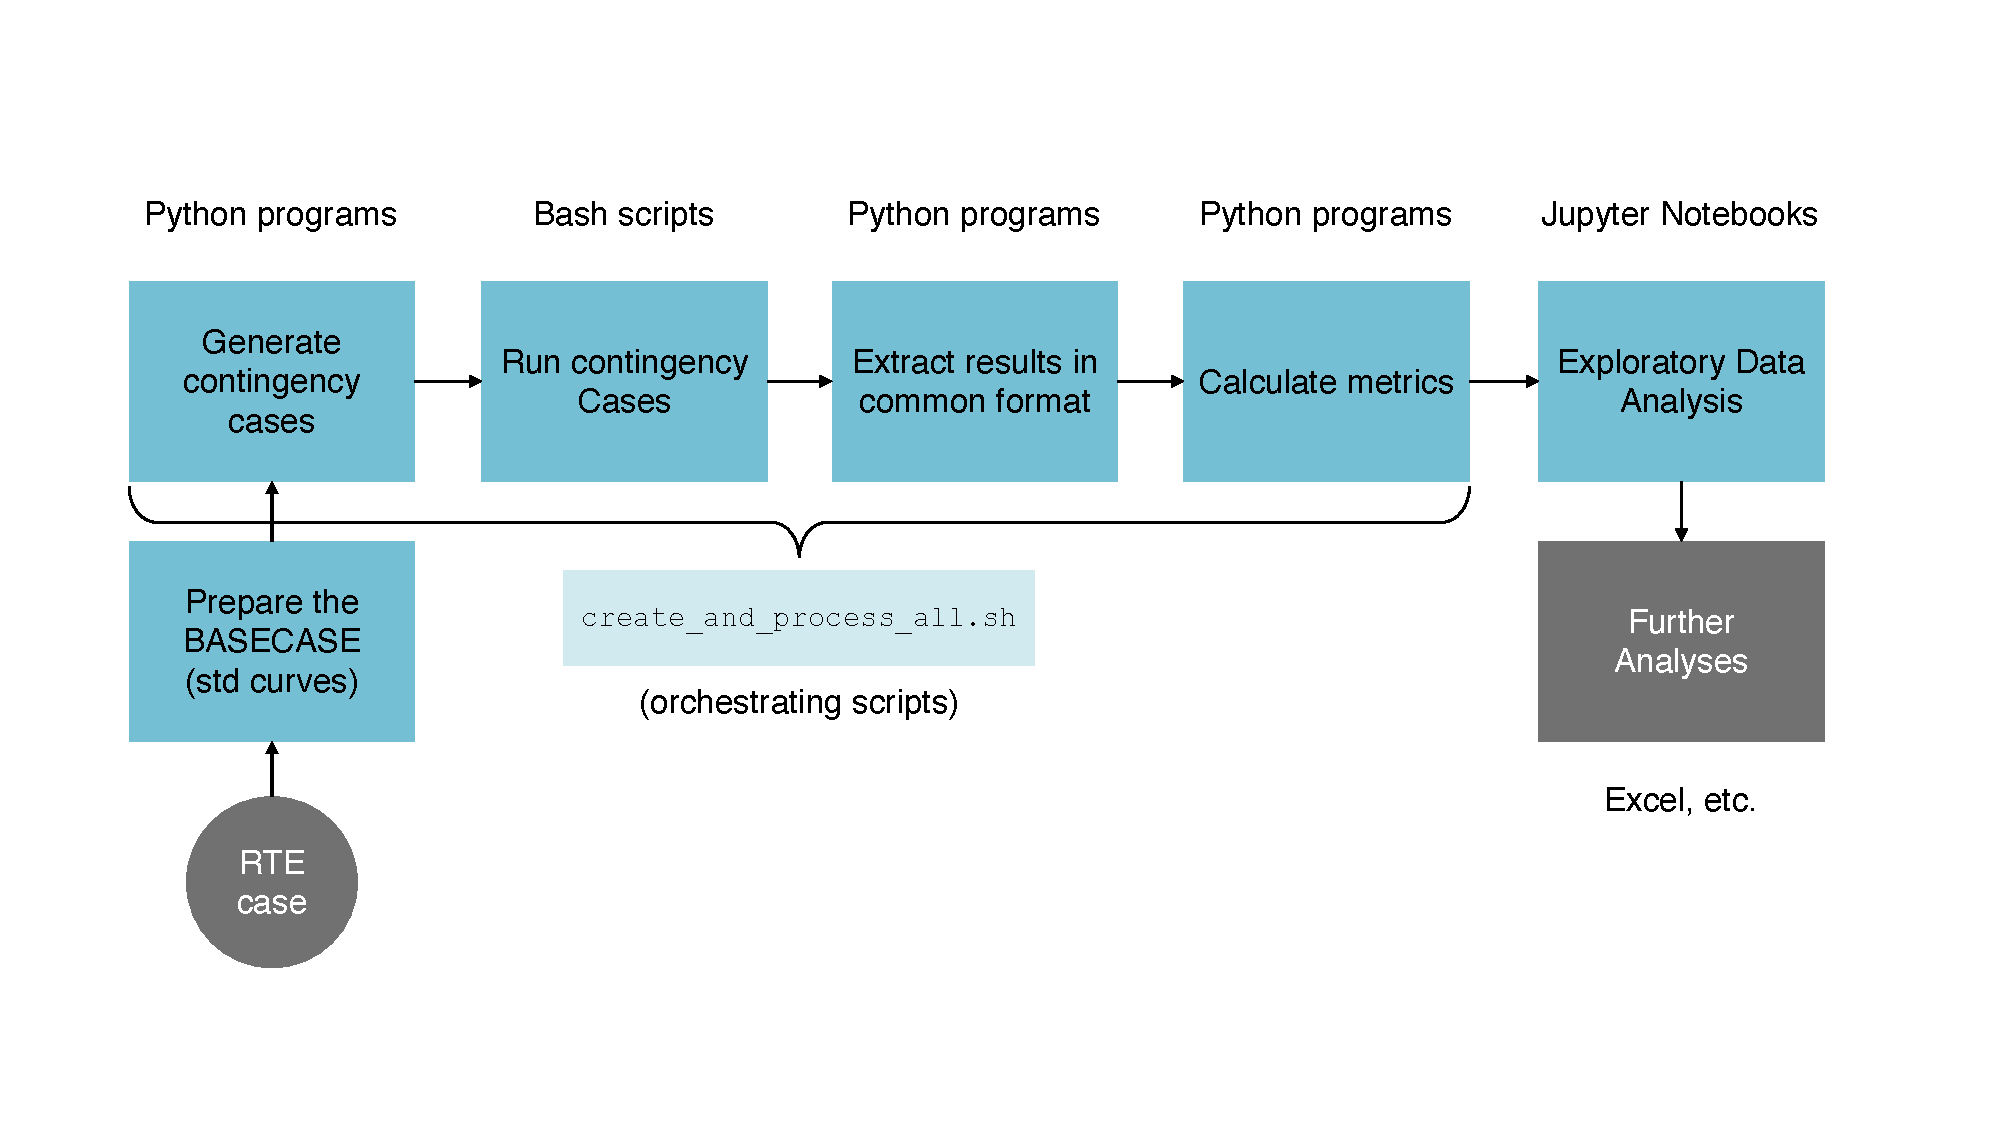
\includegraphics[width=0.9\textwidth]{figs/pipeline1}
  \caption{The processing pipeline for validating Dynawo against
    Astre, based on contingency cases.}
  \label{fig:pipeline1}
\end{figure}


\subsection{Requirements}
\label{subsec:reqmts}

In terms of input, the system requires a valid case, in which the
Astre and Dynawo should obviously correspond to the same grid model
and steady state.  They should be arranged with the following
directory structure and file names:
\begin{console}
  <INPUTCASE_DIRNAME>
  |-- Astre
  |   `-- donneesModelesEntree.xml
  |-- fic_JOB.xml
  |-- t0
  |   |-- fic_CRV.xml
  |   |-- fic_DYD.xml
  |   |-- fic_IIDM.xml
  |   `-- fic_PAR.xml
  `-- tFin
      |-- fic_CRV.xml
      |-- fic_DYD.xml
      |-- fic_IIDM.xml
      `-- fic_PAR.xml
\end{console}

The directory file names should be exactly these, otherwise there will
be several parts of the pipeline that will fail. The parent directory
name is free (it's usually the date-time of the case).

Additionally, the system expects the input case (both in Astre and
Dynawo) to contain at least one disconnection event, since this is
used as the reference to obtain the time of the event. In other words,
the scripts read \code{"event\_tEvent"} and \code{"instant"} from
the files, instead of hard-coding the typical value (which is t=300
s). This time is read from the first event, and then all events are
discarded and replaced with the new contingency event.

In terms the computational environment, these are the general
technical requirements:
\begin{description}
\item[For the computation pipeline:] \hfill
  \begin{itemize}
  \item A Linux server, preferably with 8 or more CPU cores and 64 GB
    or more of RAM\footnote{The national case has a peak RAM usage of
      around 6 GB per Dynawo run.}
  \item An up-to-date operating system such as Debian 10, Ubuntu 20.04
    LTS, or Redhat's RHEL 8 / CentOS 8. Older distributions could
    probably work as well, but haven't been tested.
  \item A working installation of Astre and Dynawo
  \end{itemize}
\item[For the data analysis:] \hfill
  \begin{itemize}
  \item a PC / laptop with 8 GB of RAM or more, running either Linux or
    Windows.
  \item a Python environment geared towards data science (NumPy,
    Pandas) and Jupyter notebook.
  \end{itemize}
\end{description}

The next section gives more details on what software packages should
be installed in order to run the validation pipeline and the notebook.




\subsection{Install instructions}

\subsubsection*{Installing the processing pipeline}

You should have a working installation of Astre and Dynawo, with only
these particular requirements:
\begin{itemize}
\item The Dynawo version should be RTE's private version, and its
  launcher should be called \code{dynawo-RTE}, and it should be in
  the \$PATH.
\item The Astre launcher should be called \code{astre} and it should
  be in the \$PATH. \textbf{IMPORTANT:} this launcher should
  additionally invoke the Python script \code{astreToCSV.py}, right
  after the execution of Astre. This script, which was provided by
  RTE, extracts the curve data from Astre's output XML into a CSV
  file, in a format similar to Dynawo's.
\end{itemize}

In our case, we used Astre V6.6.0.3 and Dynawo-RTE 1.2.1
(rev:HEAD-4bf05ee). The launcher for Dynawo was just copied to
\code{/usr/local/bin/} as \code{dynawo-RTE}, in which we only
edited the variable \code{DYNAWO\_INSTALL\_DIR} to point to our
particular installation directory. The launcher for Astre is shown
below, in abridged form. The GitHub repository contains the exact
launchers we used, as a reference (see directory \code{launchers}).


\begin{lstlisting}[language=bash]
#!/bin/bash

# Configure the variables as in Astre's "enable" script.
export THIRDPARTY_INSTALL_DIR=/opt/astre
export MOD_INSTALL_DIR=$THIRDPARTY_INSTALL_DIR/modeles
# etc.

# Launch Astre:
adnAstre2_r -xml $1 ...  # etc. etc.

# If Astre ran OK, convert the XML output curves to CSV format:
if [ $? -eq 0 ]; then
  echo -en "\nConverting output to CSV... "
  astreToCSV.py donneesModelesSortie.xml donneesModelesSortie.csv
  if [ $? -eq 0 ]; then
    echo -e "Done.\n"
  fi
fi
\end{lstlisting}

To install the validation pipeline (as well as the notebook), simply
clone the GitHub repo to any directory of your choice. Example:
\begin{console}
mkdir $HOME/work
cd $HOME/work
git clone https://github.com/dynawo/dynawo-validation-AIA.git
\end{console}

Then you need to install the following packages (and their respective
dependencies):
\begin{itemize}
\item Python 3, NumPy, Pandas, and the lxml parser
\item rsync (used for the deduplication trick in order to save on
  storage while running contingencies)
\item xz (used for compressing data files)
\item GNU parallel (used for running Astre and Dynawo jobs in parallel) 
\end{itemize}

All of these are fairly common and are available in most Linux
distributions. Here is a command that will make sure you have all
those packages and their dependencies installed (Debian/Ubuntu):
\begin{console}
  apt-get install python3 python3-numpy python3-pandas \
                  python3-lxml rsync xz-utils parallel
\end{console}



\subsubsection*{Installing the notebook environment}

You can run the notebook \code{Dynawo-Astre Comparison.ipynb} under
either Linux or Windows (as long as you have access to the result
files from the pipeline, of course). MacOS has not been tested but it
will most likely work too, as we took care of using Python's
\code{pathlib} to deal with paths throughout.

To run the notebook you will need to install:
\begin{itemize}
\item Python 3, NumPy, and Pandas
\item Jupyter Notebook
\item Plotly (version 4.10 or higher) and ipywidgets
\item seaborn, qgrid
\end{itemize}

If you are on Linux, some of these Python packages may not be directly
available as packages in the distribution, and you may have to install
them by other means. In our case, these were directly installed from
the standard Debian repositories:
\begin{console}
  apt-get install python3 python3-numpy python3-pandas \
                 jupyter python3-seaborn
\end{console}

By contrast, these other packages had to be installed under /usr/local
(via pip3) because they were either not available in Debian Buster or
not at the minimum required version:
\begin{console}
  pip3 install plotly
  pip3 install -I ipywidgets  # to override the distro's version
  pip3 install qgrid
\end{console}

\noindent\textbf{IMPORTANT NOTE ON NBEXTENSIONS:} you may have to
explicitly enable some Jupyter Notebook extensions related to the
packages above (plotly, ipywidgets, qgrid). This happens because,
depending on the installation method, some packages do not
automatically register their notebook extensions with the local
Jupyter Notebook installation. This is the case of package qgrid. To
enable the qgrid nbextension, issue this command:
\begin{console}
  jupyter nbextension enable --py --sys-prefix qgrid
\end{console}
You can list all your existing extension and their status with the
command:
\begin{console}
  jupyter nbextension list
\end{console}



\subsection{Usage of the processing pipeline}

\subsubsection*{Automated orchestration}

We will first describe here how to run the pipeline in the most
automated way possible. If you need to know how to run each stage of
the pipeline manually step-by-step, the next subsection provides the
details.

There is only one preparation step that needs to be done
semi-manually: getting the base case ready for the pipeline. If the
provided input case complies with the requirements mentioned above in
Subsection~\ref{subsec:reqmts} (namely, it should be a valid Astre and
Dynawo case with the standard directory structure), then the
preparation is accomplished with two commands, as in the following
example:
\begin{console}
  # suppose the case is contained under directory "20180423_0900":
  $DVA/xml_utils/xml_format_dir.sh 20180423_0900
  
  $DVA/contingency-validations/prepare_basecase.py \
                               20180423_0900.FORMATTED Paris
\end{console}
where \code{\$DVA} stands for the path where the GitHub code was
cloned to. The first command just re-formats all XML files so that any
edits produced by subsequent scripts (which employ the lxml parser)
produce minimal diffs; this important for auditability and quick
debugging. The second command uses the newly formatted case to produce
the actual base case for the pipeline, which in this case will be
named \code{20180423\_0900.BASECASE}.

From here onward everything is automated, using the orchestrating
script \code{create\_and\_process\_all.sh}. You should invoke this script
passing two arguments, the name of the base case directory and the
name of the directory where you want the results. For instance,
following our previous example:
\begin{console}
  $DVA/contingency-validations/create_and_process_all.sh \
                     20180423_0900.BASECASE 20180423_0900.RESULTS
\end{console}
This will run all the necessary steps of the processing pipeline:
create the contingency cases, run them, extract their results in a
common (i.e. comparable) format, and compute all metrics. It will do
so for all the device types that you enable: generators, loads, etc.
To configure which type of contingencies should be processed or
skipped, you should edit the list at the top of the script
\code{create\_and\_process\_all.sh}, in the section marked as
configurable variables. Note that running all possible types of
contingencies, and with no limit on their number, may result in quite
long runs, especially in the national grid case. You may limit the
number of contingencies via sampling, which is described below in the
subsection that shows each step of the pipeline.

You would normally launch this script and come back much later to
gather the results. If you do not want to lose the console output in
case of disconnection to the server, it is useful to launch it with
\code{nohup} and redirecting standard output and error to a file, for
later inspection:
\begin{console}
  nohup $DVA/contingency-validations/create_and_process_all.sh \
                   20180423_0900.BASECASE 20180423_0900.RESULTS \
                   > fullrun.stdout 2>&1 &
\end{console}

If you are now interested only in the analysis of results with the
notebook, you may skip the rest of this and head to
Subsection~\ref{subsec:notebook} below.



\subsubsection*{The output files in detail}

The results from the processing pipeline are compressed and structured
in directories, as follows.  Suppose for instance that we enabled only
shunt, generator, and branch contingencies (on both sides). At the end
of the run, we would obtain the following:
\begin{console}
  tree -d  20180423_0900.RESULTS
  
  20180423_0900.RESULTS
  |-- branchBs
  |   |-- aut
  |   |-- casediffs
  |   |-- crv
  |   |-- log
  |   |-- metrics
  |   `-- xml
  |-- gens
  |   |-- aut
  |   |-- casediffs
  |   |-- crv
  |   |-- log
  |   |-- metrics
  |   `-- xml
  `-- shunts
      |-- aut
      |-- casediffs
      |-- crv
      |-- log
      |-- metrics
      `-- xml
\end{console}

The key results are left under the \code{metrics} directories; this is
the data that constitutes the main input for the Jupyter notebook, for
the analysis of results. The rest of the directories are also
important for audit purposes and debugging. Briefly:
\begin{description}
\item[\code{aut}] Contains the automata changes extracted from Astre
  and Dynawo output (in unified normalized form). These are analogous
  to the CRV files, but for automata events instead of continuous
  magnitudes.
\item[\code{casediffs}] Contains the contingency cases, compresses as
  unified diffs. You may easily reconstruct the actual contingency
  case from these diffs and the base case (quick instructions in the
  \code{README} file inside).
\item[\code{crv}] Contains the CRV files obtained from Astre and
  Dynawo. Note that they already contain the same column order and
  variable names thanks to the preparation step
  (\code{prepare\_basecase.py}).
\item[\code{log}] Contains the Astre and Dynawo log files produced in
  the simulation run, as well as their respective standard output to
  the console (the \code{*.runStdout.*} files).
\item[\code{metrics}] The computed metrics, used by the notebook for
  analysis.
\item[\code{xml}] Contains all other output produced by Astre and
  Dynawo, for total auditability of results. This includes the full
  Sortie file from Astre, plus the Constraints, OutputIIDM, and
  TimeLine from Dynawo.
\end{description}

Note that most data files are compressed with \code{xz}, for efficient
use of the storage. Nevertheless, it is quite easy to inspect and
search them with the \code{xz} tools (\code{xzcat, xzcmp, xzdiff,
  xzgrep, xzless}). Processing them with Python Pandas is also
transparent.



\subsubsection*{Manually, step by step}

We now describe how to run the pipeline step by step, which is useful
to get acquainted with the inner workings of the system and be able to
debug it when something goes wrong. We will label the steps as we did
in the introduction above in
Subsection~\ref{subsec:hl_intro}. Figure~\ref{fig:pipeline2} will also
help in visualizing all the steps in terms of the scripts and programs
that drive them.

\begin{figure}
  \centering
  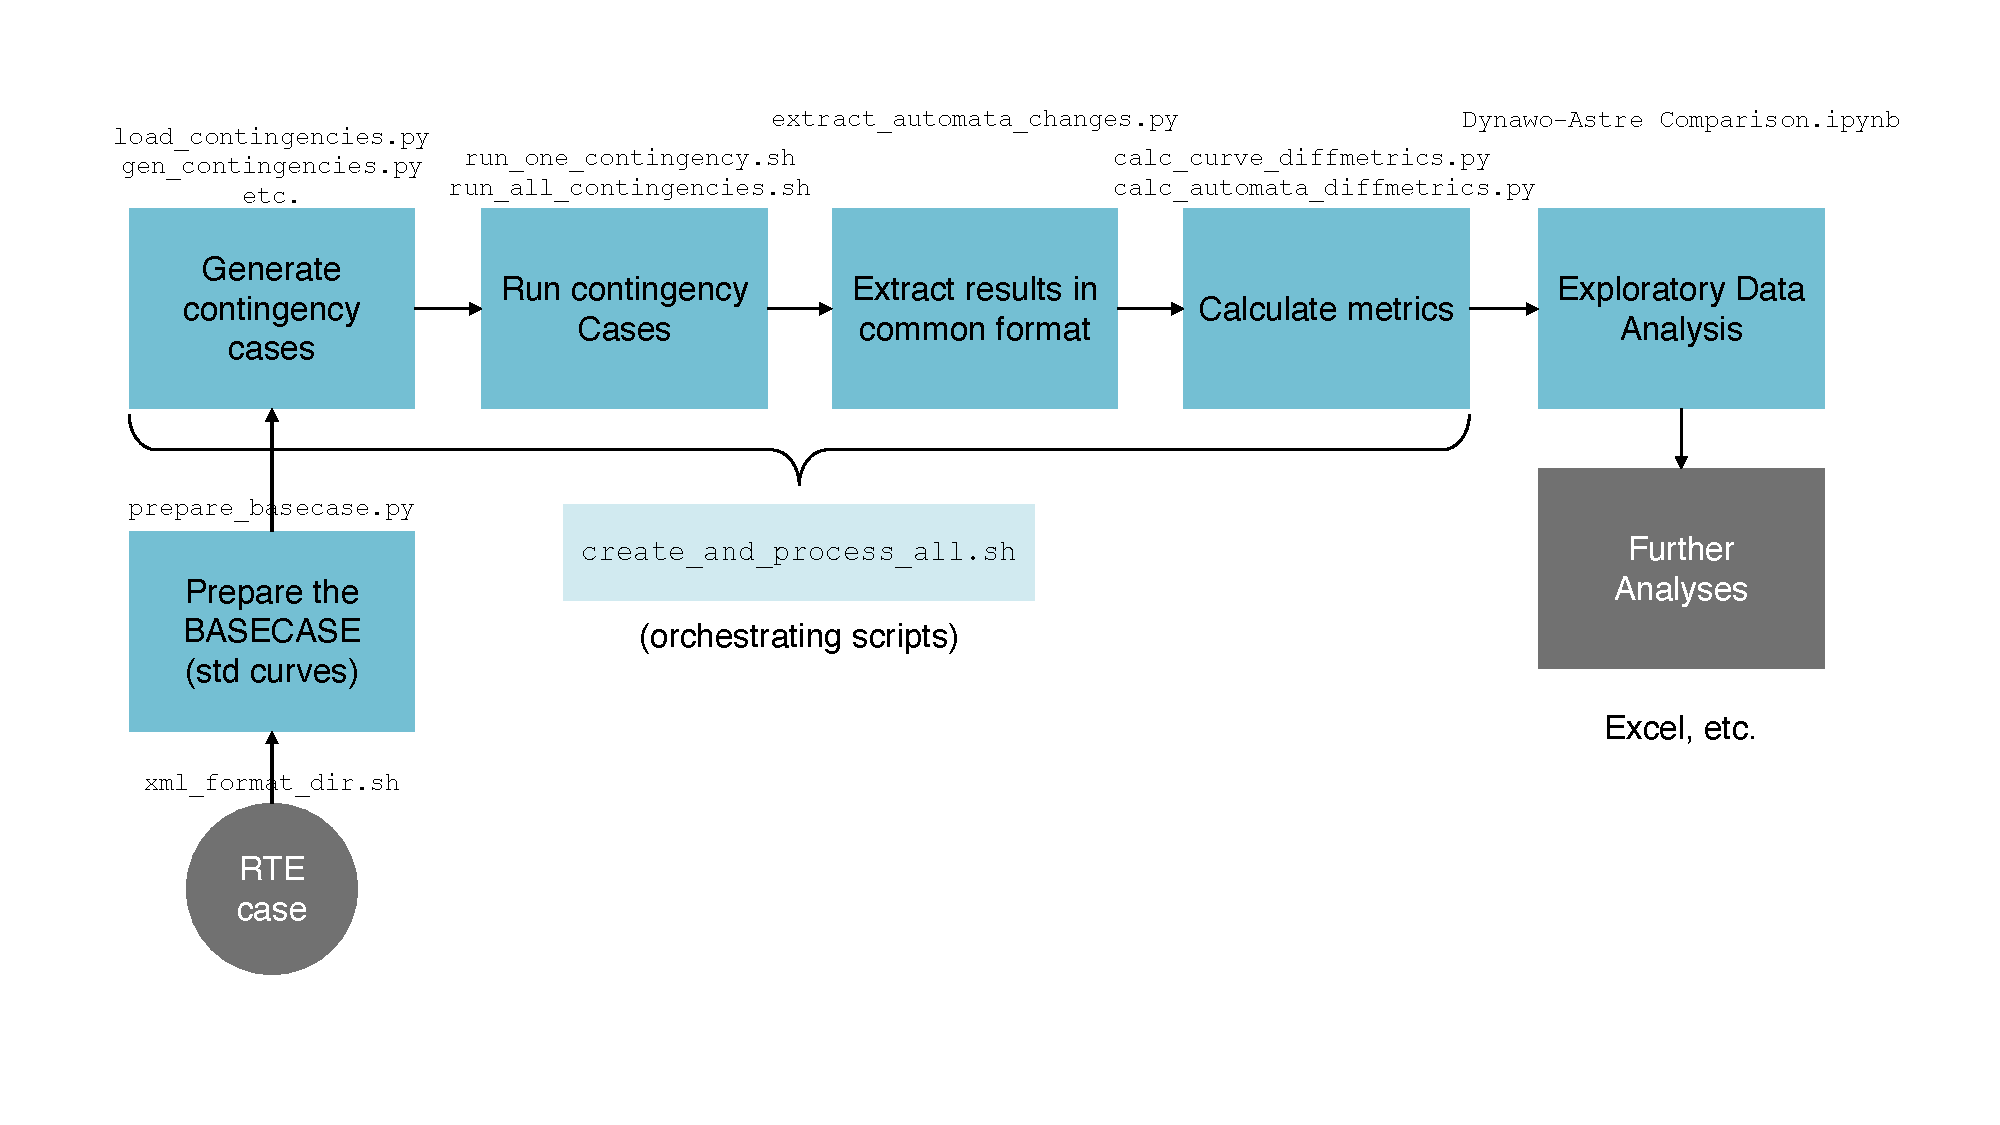
\includegraphics[width=0.9\textwidth]{figs/pipeline2}
  \caption{The processing pipeline: names of the Bash scripts and
    Python programs involved.}
  \label{fig:pipeline2}
\end{figure}

\noindent\textbf{Step 1:} Obtaining the input a study case. It just
needs to satisfy the minimal requirements we mentioned in
Subsection~\ref{subsec:reqmts} above (validity, structure, and
containing at least one event).

\noindent\textbf{Step 2} Preparing the base case: Python program
\code{prepare\_basecase.py}.  Also described in the previous
subsection, this is done for standardizing the XML format (which
ensures minimal diffs) and for standardizing the curves to be
extracted (which ensures that the curve outputs in Astre and Dynawo
are directly comparable, having the same variable names).

\noindent\textbf{Step 3} Create the contingency cases derived from the
base case: Python programs \code{shunt\_contingencies.py,
  load\_contingencies.py, etc.}. They are all run in the same way,
passing one mandatory argument (the directory containing the base
case) and optionally a list of one or more element names to
process. If no elements are given, the program will generate all
possible matched elements between the Astre and Dynawo files.  If run
with no arguments at all, the program will show a reminder of how it
should be invoked:
\begin{console}
  $DVA/contingency-validations/loads/load_contingencies.py 

  Usage: load_contingencies.py base_case [element1 element2 ...]
\end{console}
(All Python and Bash scripts provide this kind of quick help message.)
This step of the pipeline is the one that can potentially generate too
many files and end up filling up the disk. To minimize this risk, the
program uses a file ``deduplication'' technique in order to save space
for each contingency, whereby only the files that are really different
from the base case are the ones that take up space---the rest are hard
links to the base case. Still, cases like the National grid case may
generate files in excess of several hundred GB (branch contingencies,
for instance, generate a total of 9,437 cases, which yields a peak of
about 550 GB). This is only temporary because the final results are
compressed and end up taking up less than 20 times that space, but
this may still be a practical problem some times. To cope with this,
these Python programs also offer the possibility of limiting the
number of contingencies to a \emph{random sample} of all possible
matches. This is done by editing the variable \code{MAX\_NCASES} at
the top of each script; you only need to choose a maximum number of
contingency cases and the code will adapt its random sampling rate so
that the final number of cases is around that number (plus-minus some
variation due to the randomness).

\noindent\textbf{Step 4} Run Astre and Dynawo on the contingency
cases: Bash scripts \code{run\_one\_contingency.sh} and
\code{run\_all\_contingencies.sh}. These run the cases generated in
the previous step, collecting logs and results into organized and
highly compressed storage. To get a quick reminder about usage and
options, just execute the scripts without any parameters. The script
\code{run\_one\_contingency.sh} is the real workhorse: it creates the
directory structure for the output, it stores the contingency case in
``diff'' form, runs both Astre and Dynawo (stopping if there are any
errors), collects and compresses all possible results (not just the
curves) using \code{xz}, and finally extracts the relevant automata
events (taps, shunts) in a common format. Optionally, it deletes the
contingency case at the end of the run, once all output has been
collected. The \code{run\_all\_contingencies.sh} script, on the other
hand, is just used to repeatedly call on
\code{run\_one\_contingency.sh}, until all the contingency cases
(those created in the previous step) have been processed. Its major
role is enabling the selection of \emph{sequential} or \emph{parallel}
(the default) execution of contingency jobs. Here is a typical example
of launching this script:
\begin{console}
  $DVA/contingency-validations/run_all_contingencies.sh \
                     -c -v -o 20180423_0900.RESULTS/shunts \
                     . 20180423_0900.BASECASE shunt_
\end{console}
where, as before, \code{\$DVA} represents the location where the
GitHub code was cloned to. Note that the first non-option parameter
(in this example, the current directory, \code{"."}) is the directory
where all contingency cases have been created in Step 3. The third and
last parameter is just the prefix of the contingencies.  When in
doubt, just execute the script with no parameters and you will get a
quick reminder on its usage.

\noindent\textbf{Step 5} Extract result data (automata events) in a
format common to Astre and Dynawo: Python program
\code{extract\_automata\_changes.py}.  This step is actually executed
as part of Step 4 (invoked as the last step in script
\code{run\_one\_contingency.sh}), but it is mentioned here in case it
needs to be run on its own, for debugging or auditing purposes. To run
it, simply execute it passing one argument, the name of a contingency case for
which Astre and Dynawo have already been run. The program only focuses
on automata events, because curve data have already been standardized
thanks to Step 2 (\code{prepare\_basecase.py}).

\noindent\textbf{Step 6} Compute metrics on the results obtained, both
for curves and for selected automata events: Python programs
\code{calc\_curve\_diffmetrics.py} and
\code{calc\_automata\_diffmetrics.py}, respectively. To launch the
calculation of curve metrics, you have to pass the directory where the
curves files were collected and the prefix used for the contingency
type (the device). For instance, assuming we have shunt contingencies
already collected under directory \code{20180423\_0900.RESULTS/shunts}:
\begin{console}
  $DVA/metrics/calc_curve_diffmetrics.py \
                  20180423_0900.RESULTS/shunts/crv  shunt_
\end{console}
and for automata event metrics, the call would be:
\begin{console}
  $DVA/metrics/calc_automata_diffmetrics.py \
                  20180423_0900.RESULTS/shunts/aut  shunt_ \
                  20180423_0900.BASECASE
\end{console}
Note that in this case the automata diff-metrics script also needs to
be passed the location of the BASE CASE, as it needs to read the Astre
and Dynawo files in order to construct certain auxiliary data
structures.  The results from both of these scripts are left under
directory \code{../metrics}, relative to the curve and automata data
(in this example, that would be
\code{20180423\_0900.RESULTS/shunts/metrics}).




\subsection{Usage of the Jupyter notebook}
\label{subsec:notebook}

\subsubsection{Running the notebook}

The Jupyter notebook is provided as two files:
\begin{itemize}
\item \code{Dynawo-Astre Comparison.maincode.py}
\item \code{Dynawo-Astre Comparison.template.ipynb}
\end{itemize}
The first one, as its name suggests, is pure Python code containing
functions and cell code used by the notebook (in fact, it is designed
to get included verbatim by the notebook). The second one is the base
template for the actual notebook. To use it, just copy it to any other
name, in any directory of your choice, and then edit the two variables
at the top cell:
\begin{lstlisting}[language=python]
  # Case selection (adapt CRV_DIR as needed)
  CRV_DIR = '/work/PtFige-Paris/20180423_0900.RESULTS/shunts/crv'
  PREFIX = 'shunt_'
\end{lstlisting}
There is also a utility script called \code{generate\_notebooks.py}
that you may use in order to automatically generate several notebooks
in one go. This is useful in case you have many combinations of cases
and contingency types to explore. For instance:
\begin{console}
  $ ./generate_notebooks.py /work/PtFige-Paris *RESULTS
  Generating notebook: PtFige-Paris_20180423_0900.RESULTS_gens.ipynb
  Generating notebook: PtFige-Paris_20180423_0900.RESULTS_loads.ipynb
  Generating notebook: PtFige-Paris_20180423_0900.RESULTS_shunts.ipynb
\end{console}
this will generate three notebooks, each with the correct values of
the variables \code{CRV\_DIR} and \code{PREFIX}.

To run the notebook for the first time, you have to run all cells
\emph{twice}. This is because the first time it is run it will only
execute the ``magic'' command that loads the main code.  From there
on, you can always re-run it by executing \emph{Cell $\rightarrow$ Run
  All} from the menu. Actually, given the non-linear nature of
notebooks, it's recommended to always run \emph{Kernel $\rightarrow$
  Restart \& Run All}, to make sure that all cells are run starting
from a clean state and in the expected order.


\subsubsection{Exploring the results}

Once you have run the complete notebook you can analyze the
results. The notebook is structured in these main sections:
\begin{description}
\item[Summary section:] summary percentages of cases that pass the
  threshold criteria (both including and excluding cases that are
  \emph{unstable}, either pre- or post-contingency).
\item[Scores by measure:] A sortable grid table showing scores by
  measure, that is, by any combination of contingency case and
  (curve) variable.
\item[Graphs by measure:] A group of three graphs that allows
  inspecting and comparing results in detail, down to the level of the
  individual variable and contingency case (for both curves and
  automata changes).
\item[Scores by contingency:] A sortable grid table showing scores by
  contingency. It's similar to the former grid, but this one
  contemplates the metrics derived from automata events and
  additionally it incorporates a couple of boolean marks that show
  whether or not the case as a whole can be considered \emph{stable}
  (pre- or post-contingency).
\item[Heatmap graph for contingencies:] A simple heatmap of all the
  defined scores, which shows at a glance which contingency cases are
  the most problematic.
\end{description}
Please refer to Section~\ref{sec:metrics} above for all the details
about how the metrics are defined and what are the thresholds used for
defining the pass/not-pass criteria.


[TODO: Add a description here in more detail of each of these graphics
  and tables, including relevant screenshots.]






\section{Dynawo validation pipeline: Developer Notes}
\label{sec:devnotes}
[TODO]







\appendix
\section{GitHub repository}
\label{app:github}
[TODO: brief description of the GitHub repo structure, and pointers to the docs in there.]
      


\end{document}




%%% Example snapshot of Dynawo under iotop:
%% \begin{console}
%% Total DISK READ:         0.00 B/s | Total DISK WRITE:      1615.07 K/s
%% Current DISK READ:       0.00 B/s | Current DISK WRITE:    1301.64 K/s
%%   TID  PRIO  USER     DISK READ  DISK WRITE  SWAPIN     IO>    COMMAND
%% 23046 be/4 marinjl     0.00 B/s  173.31 K/s  0.00 % 95.32 % dynawo fic_JOB.xml
%% 22780 be/4 marinjl     0.00 B/s  180.68 K/s  0.00 % 95.31 % dynawo fic_JOB.xml
%% 23069 be/4 marinjl     0.00 B/s  176.99 K/s  0.00 % 94.40 % dynawo fic_JOB.xml
%% 22707 be/4 marinjl     0.00 B/s  176.99 K/s  0.00 % 94.18 % dynawo fic_JOB.xml
%% 23056 be/4 marinjl     0.00 B/s  176.99 K/s  0.00 % 92.25 % dynawo fic_JOB.xml
%% 23076 be/4 marinjl     0.00 B/s  176.99 K/s  0.00 % 91.83 % dynawo fic_JOB.xml
%% 22616 be/4 marinjl     0.00 B/s  221.24 K/s  0.00 % 97.43 % dynawo fic_JOB.xml
%% 22623 be/4 marinjl     0.00 B/s  188.06 K/s  0.00 % 92.98 % dynawo fic_JOB.xml
%% \end{console}



%% \begin{figure}
%%   \centering
%%   \includegraphics[width=\columnwidth]{figs/myfig}
%%   \caption{Blah...}
%%   \label{fig:blah}
%% \end{figure}

%% \begin{table}[!t]
%%   \centering
%%   %% increase table row spacing, adjust to taste
%%   %\renewcommand{\arraystretch}{1.3}
%%   % if using array.sty, it might be a good idea to tweak the value of
%%   % \extrarowheight as needed to properly center the text within the cells
%%   %% Some packages, such as MDW tools, offer better commands for making tables
%%   %% than the plain LaTeX2e tabular which is used here.
%%   \begin{tabular}{lccc}
%%     \hline
%%     \noalign{\smallskip}
%%     Pad\'e order & $\sigma=-0.07-j0.08$ & $-0.14-j0.15$ & $-0.2-j0.22$ \\
%%     & ($|V|=0.92$) & ($|V|=0.81$) &($|V|=0.58$)\\
%%     \noalign{\smallskip}
%%     \hline
%%     \noalign{\smallskip}
%%     [2/2] & 1.795e-03 & 2.30e-02 & 2.74e-01 \\
%%     {}[5/5] & 7.02e-09 & 2.10e-05 & 5.85e-02 \\
%%     {}[10/10] & 0 & 1.89e-10 & 1.16e-02 \\
%%     {}[15/15] & 0 & 1.55e-15 & 2.86e-03 \\
%%     {}[20/20] & 0 & 0 & 7.38e-04 \\
%%     \noalign{\smallskip}
%%     \hline
%%   \end{tabular}
%%   \caption{Examples of relative precision of Pad\'e Approximants vs. order.}
%%   \label{tbl:padecalc}
%% \end{table}
